\documentclass[11pt,a4paper]{article}

% Packages
\usepackage[utf8]{inputenc}
\usepackage[T1]{fontenc}
\usepackage{geometry}
\usepackage{xcolor}
\usepackage{graphicx}
\usepackage{booktabs}
\usepackage{tabularx}
\usepackage{titlesec}
\usepackage{fancyhdr}
\usepackage{tikz}
\usepackage{pgfplots}
\usepackage{tcolorbox}
\usepackage{amsmath}
\usepackage{amssymb}
\usepackage{enumitem}

% Configuration
\geometry{top=2.5cm, bottom=2.5cm, left=2cm, right=2cm}
\pgfplotsset{compat=1.18}
\usetikzlibrary{arrows.meta, positioning, calc}

% Colors
\definecolor{primary}{HTML}{1A237E}
\definecolor{accent}{HTML}{0D47A1}
\definecolor{muted}{HTML}{546E7A}
\definecolor{chart1}{HTML}{2196F3}
\definecolor{chart2}{HTML}{00BCD4}
\definecolor{chart3}{HTML}{4CAF50}
\definecolor{chart4}{HTML}{FFC107}
\definecolor{chart5}{HTML}{FF5722}

% Custom Commands
\newcommand{\InstituteName}{Global Institute of Technology \& Management}
\newcommand{\ReportTitle}{Annual Institutional Performance Report 2023-24}
\newcommand{\ReportDate}{October 2024}
\newcommand{\rupee}{Rs.~}

\newcommand{\kpi}[2]{
    \begin{tcolorbox}[colback=gray!5, colframe=gray!10, arc=5pt, boxrule=0.5pt, halign=center]
        {\footnotesize\uppercase{\textcolor{muted}{#1}}}\\[0.1cm]
        {\Large\textbf{\textcolor{primary}{#2}}}
    \end{tcolorbox}
}

\newenvironment{card}{
    \begin{tcolorbox}[colback=white, colframe=gray!20, arc=5pt, boxrule=0.5pt, left=15pt, right=15pt, top=15pt, bottom=15pt]
}{
    \end{tcolorbox}
}

% Header/Footer
\pagestyle{fancy}
\fancyhf{}
\fancyhead[L]{\textcolor{muted}{\small \InstituteName}}
\fancyhead[R]{\textcolor{muted}{\small \ReportTitle}}
\fancyfoot[C]{\thepage}
\renewcommand{\headrulewidth}{0.4pt}
\renewcommand{\footrulewidth}{0pt}

\begin{document}

% --- COVER PAGE ---
\thispagestyle{empty}
\begin{center}
    \vspace*{2cm}
    
\begin{tikzpicture}
        \fill[primary] (0,0) circle (1.5cm);
        \node at (0,0) {\textcolor{white}{\Huge\textbf{G}}};
    \end{tikzpicture}
    
    \vspace{1.5cm}
    {\Huge\textcolor{primary}{\textbf{\ReportTitle}}}\\[0.5cm]
    {\Large\textcolor{muted}{\InstituteName}}\\[0.2cm]
    {\large \ReportDate}
    
    \vspace{2cm}
    
    \begin{card}
        \section*{Executive Summary}
        The academic year 2023-24 has been a landmark period for the \InstituteName. We have seen a 15\% increase in student enrollment, driven by our new programs in Artificial Intelligence and Data Science. Our placement cell achieved a record-breaking 94.2\% placement rate, with the highest package reaching \rupee 45 LPA. Research output has grown by 22\%, with faculty members securing significant grants from national agencies. This report details our progress across academic, career, research, and financial domains.
    \end{card}
    
    \vspace{1cm}
    
    \begin{minipage}[t]{0.31\textwidth}
        \kpi{Student Enrollment}{4,850}
    \end{minipage}%
    \hfill
    \begin{minipage}[t]{0.31\textwidth}
        \kpi{Placement Rate}{94.2\%}
    \end{minipage}%
    \hfill
    \begin{minipage}[t]{0.31\textwidth}
        \kpi{Research Pubs}{342}
    \end{minipage}
\end{center}
\clearpage

% --- SECTION 1: ACADEMIC ---
\section*{Academic Excellence and Enrollment Trends}
{\large\textcolor{muted}{Analysis of student growth and departmental performance}}

\vspace{0.5cm}

\begin{card}
    The institution has maintained a steady upward trajectory in student recruitment and academic retention. The introduction of specialized tracks in emerging technologies has attracted a diverse cohort of students from across the country. Our faculty-to-student ratio remains at a competitive 1:15, ensuring personalized mentorship and high academic standards.
    
    \vspace{0.8cm}
    
    \begin{center}
    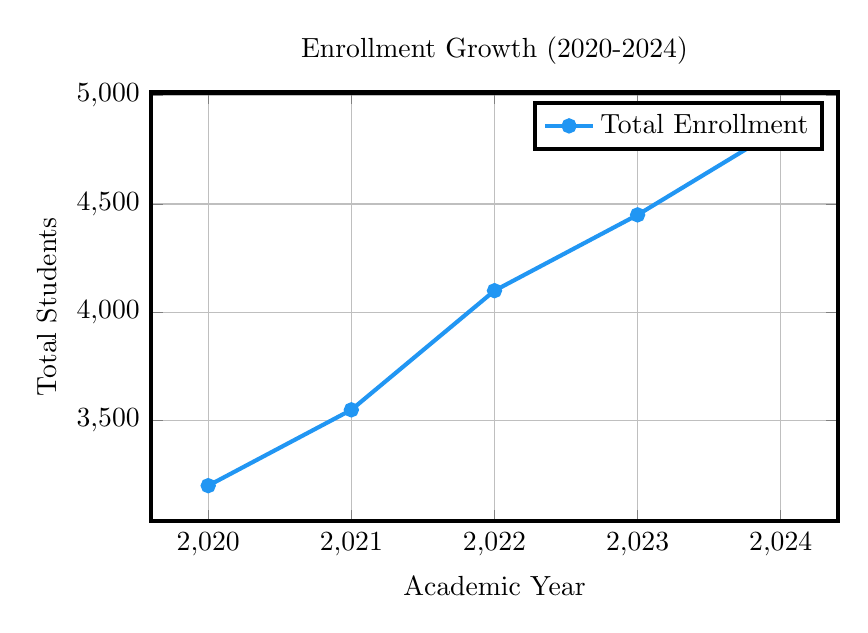
\begin{tikzpicture}
    \begin{axis}[
        width=0.85\textwidth,
        height=200pt,
        xlabel={Academic Year},
        ylabel={Total Students},
        grid=major,
        line width=1.5pt,
        title={Enrollment Growth (2020-2024)},
        xtick={2020,2021,2022,2023,2024},
        tick label style={/pgf/number format/fixed, /pgf/number format/precision=0},
    ]
    \addplot[color=chart1, mark=*, line width=1.5pt] coordinates {
        (2020,3200) (2021,3550) (2022,4100) (2023,4450) (2024,4850)
    };
    \legend{Total Enrollment}
    \end{axis}
    \end{tikzpicture}
    \end{center}
\end{card}

\vspace{0.5cm}

\begin{card}
    \subsection*{Departmental Performance Metrics}
    \vspace{0.3cm}
    \begin{tabularx}{\textwidth}{@{}lXrr@{}}
        \toprule
        \textbf{Department} & \textbf{Enrollment} & \textbf{Pass Percentage} & \textbf{Avg. GPA} \\
        \midrule
        Computer Science \& Eng. & 1,200 & 98.2\% & 8.4 \\
        Electronics \& Comm. & 950 & 94.5\% & 7.9 \\
        Mechanical Engineering & 800 & 89.1\% & 7.2 \\
        Civil Engineering & 650 & 87.4\% & 7.1 \\
        Management Studies (MBA) & 1,250 & 96.8\% & 8.1 \\
        \bottomrule
    \end{tabularx}
\end{card}

\clearpage

% --- SECTION 2: CAREER ---
\section*{Career Services and Placement Outcomes}
{\large\textcolor{muted}{Employment statistics and industry engagement}}

\vspace{0.5cm}

\begin{card}
    Our Career Development Cell (CDC) has successfully bridged the gap between academia and industry. This year, we hosted over 150 recruiting partners, including Fortune 500 companies and high-growth startups. The average salary package has seen a significant jump from \rupee 7.8 LPA to \rupee 8.5 LPA.
    
    \vspace{0.8cm}
    
    \begin{minipage}[t]{0.48\textwidth}
        \centering
        \textbf{Placement by Sector}\\
        \vspace{0.5cm}
        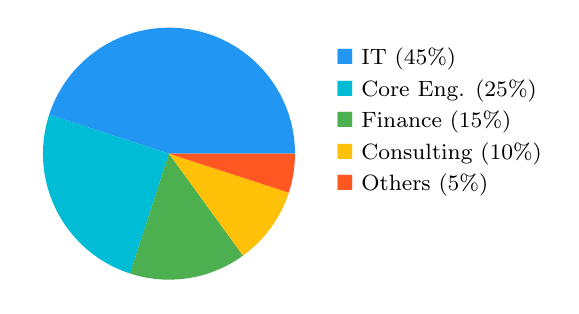
\begin{tikzpicture}[scale=0.8]
            \def\radius{2cm}
            \fill[chart1] (0,0) -- (0:\radius) arc (0:162:\radius) -- cycle;
            \fill[chart2] (0,0) -- (162:\radius) arc (162:252:\radius) -- cycle;
            \fill[chart3] (0,0) -- (252:\radius) arc (252:306:\radius) -- cycle;
            \fill[chart4] (0,0) -- (306:\radius) arc (306:342:\radius) -- cycle;
            \fill[chart5] (0,0) -- (342:\radius) arc (342:360:\radius) -- cycle;
            
            \node[anchor=west] at (2.5, 1.5) {\footnotesize\textcolor{chart1}{$\blacksquare$} IT (45\%)};
            \node[anchor=west] at (2.5, 1.0) {\footnotesize\textcolor{chart2}{$\blacksquare$} Core Eng. (25\%)};
            \node[anchor=west] at (2.5, 0.5) {\footnotesize\textcolor{chart3}{$\blacksquare$} Finance (15\%)};
            \node[anchor=west] at (2.5, 0.0) {\footnotesize\textcolor{chart4}{$\blacksquare$} Consulting (10\%)};
            \node[anchor=west] at (2.5, -0.5) {\footnotesize\textcolor{chart5}{$\blacksquare$} Others (5\%)};
        \end{tikzpicture}
    \end{minipage}%
    \hfill
    \begin{minipage}[t]{0.48\textwidth}
        \centering
        \textbf{Average Salary Trend (\rupee LPA)}\\
        \vspace{0.5cm}
        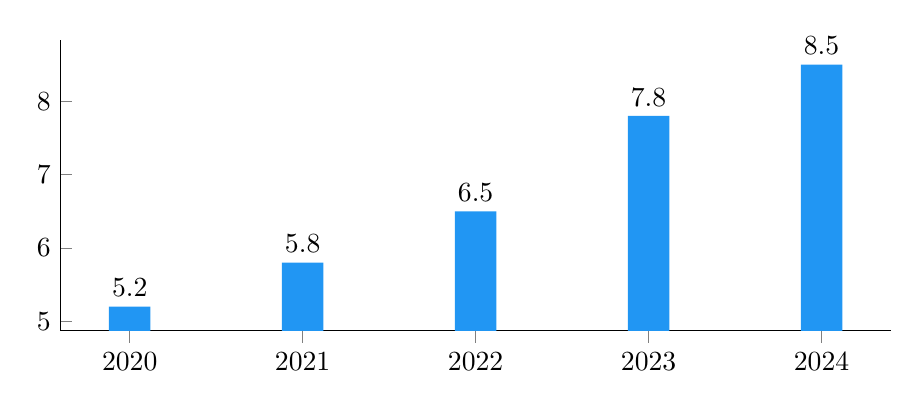
\begin{tikzpicture}
        \begin{axis}[
            ybar,
            width=\textwidth,
            height=150pt,
            symbolic x coords={2020,2021,2022,2023,2024},
            xtick=data,
            bar width=15pt,
            nodes near coords,
            axis lines*=left,
        ]
        \addplot[fill=chart1, draw=none] coordinates {
            (2020,5.2) (2021,5.8) (2022,6.5) (2023,7.8) (2024,8.5)
        };
        \end{axis}
        \end{tikzpicture}
    \end{minipage}
\end{card}

\vspace{0.5cm}

\begin{card}
    \subsection*{Top Recruiting Partners 2024}
    \vspace{0.3cm}
    \begin{tabularx}{\textwidth}{@{}lXrr@{}}
        \toprule
        \textbf{Company} & \textbf{Sector} & \textbf{Students Hired} & \textbf{Package (\rupee LPA)} \\
        \midrule
        Google & Technology & 12 & 45.0 \\
        Microsoft & Technology & 8 & 42.5 \\
        TCS & IT Services & 145 & 7.5 \\
        Infosys & IT Services & 112 & 6.8 \\
        Deloitte & Consulting & 45 & 12.5 \\
        HDFC Bank & Finance & 38 & 9.2 \\
        \bottomrule
    \end{tabularx}
\end{card}

\clearpage

% --- SECTION 3: RESEARCH ---
\section*{Research, Innovation, and Intellectual Property}
{\large\textcolor{muted}{Scholarly output and external funding}}

\vspace{0.5cm}

\begin{card}
    The institution has fostered a robust research culture, resulting in a 22\% year-on-year growth in publications. Our faculty members have been actively involved in interdisciplinary research, particularly in the fields of sustainable energy and healthcare AI.
    
    \vspace{0.8cm}
    
    \begin{center}
    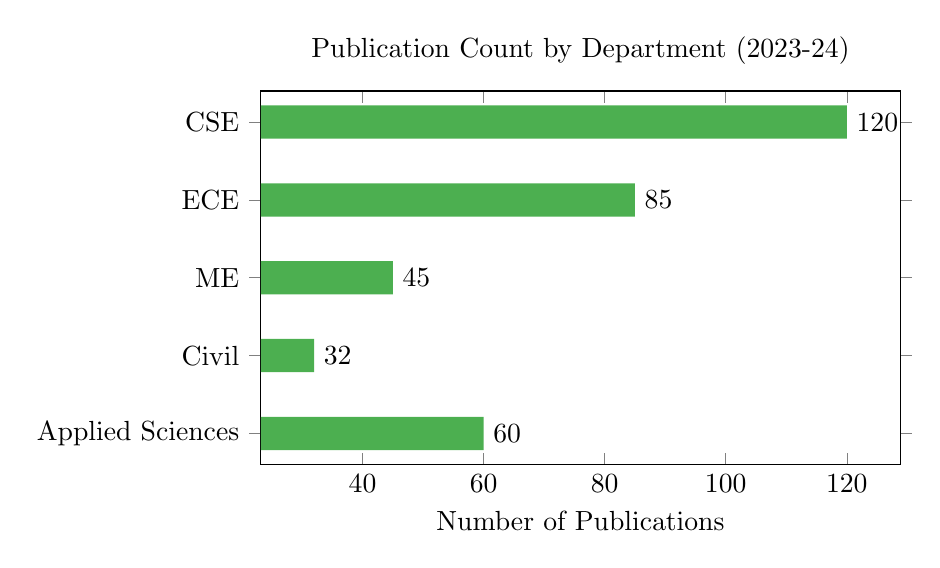
\begin{tikzpicture}
    \begin{axis}[
        xbar,
        width=0.8\textwidth,
        height=180pt,
        symbolic y coords={Applied Sciences,Civil,ME,ECE,CSE},
        ytick=data,
        xlabel={Number of Publications},
        title={Publication Count by Department (2023-24)},
        bar width=12pt,
        nodes near coords,
    ]
    \addplot[fill=chart3, draw=none] coordinates {
        (120,CSE) (85,ECE) (45,ME) (32,Civil) (60,Applied Sciences)
    };
    \end{axis}
    \end{tikzpicture}
    \end{center}
\end{card}

\vspace{0.5cm}

\begin{card}
    \subsection*{Research Grants and Funding}
    \vspace{0.3cm}
    \begin{tabularx}{\textwidth}{@{}lXrr@{}}
        \toprule
        \textbf{Funding Agency} & \textbf{Project Title} & \textbf{Amount (\rupee Lakhs)} \\
        \midrule
        DST & AI-driven Diagnostic Tools for Rural Healthcare & 45.5 \\
        SERB & Quantum Computing Algorithms for Cryptography & 32.0 \\
        ISRO & Satellite Communication in High-Altitude Regions & 28.5 \\
        Industry Partner & Smart Grid Optimization using IoT & 15.0 \\
        \bottomrule
    \end{tabularx}
\end{card}

\clearpage

% --- SECTION 4: FINANCIAL ---
\section*{Financial Performance and Infrastructure}
{\large\textcolor{muted}{Revenue distribution and capital expenditure}}

\vspace{0.5cm}

\begin{card}
    The financial health of the institution remains strong, with a total revenue of \rupee 124 Cr for the fiscal year. We have allocated 35\% of our budget towards infrastructure development, including the completion of the new Innovation Hub and the expansion of the Central Library.
    
    \vspace{0.5cm}
    
    \begin{minipage}[t]{0.31\textwidth}
        \kpi{Total Revenue}{\rupee 124 Cr}
    \end{minipage}%
    \hfill
    \begin{minipage}[t]{0.31\textwidth}
        \kpi{Infra Investment}{\rupee 43.4 Cr}
    \end{minipage}%
    \hfill
    \begin{minipage}[t]{0.31\textwidth}
        \kpi{Scholarships}{\rupee 8.2 Cr}
    \end{minipage}
    
    \vspace{0.8cm}
    
    \textbf{Key Financial Highlights:}
    \begin{itemize}[label=\textcolor{primary}{$\bullet$}]
        \item 12\% increase in non-tuition revenue through consultancy and executive education.
        \item Operational efficiency improved by 8\% through digital transformation of administrative processes.
        \item Endowment fund reached a milestone of \rupee 25 Cr.
    \end{itemize}
\end{card}

\vspace{2cm}

\begin{center}
    \textcolor{muted}{\small --- End of Report ---}\\
    \vspace{0.2cm}
    \textcolor{muted}{\footnotesize Generated on \today}
\end{center}

\end{document}